\documentclass[italian,12pt,a4paper,oneside,final]{report}
%\documentclass[italian,a4paper,titlepage]{article}
%\usepackage{amsmath}
%\usepackage{caption}
%\usepackage{subcaption}
\usepackage{graphicx}
\usepackage{biblatex} %Imports biblatex package
\usepackage[utf8]{inputenc}
\usepackage[italian]{babel}
\usepackage{csquotes}
%\usepackage[T1]{fontenc}
%\usepackage{longtable}
%\usepackage{booktabs}
%\usepackage{textcomp}
\usepackage[draft=false]{hyperref}
%\usepackage{hyperref}
%\usepackage[table]{xcolor}
\addbibresource{iot.bib} %Import the bibliography file
\graphicspath{ {images/} }
\renewcommand{\thesection}{\arabic{section}} % remove the \chapter counter from being printed with every \section
\hypersetup{
	colorlinks=true,
	linkcolor=,
	pdftitle={Marco Giunta - Progetto IoT},
	pdfauthor={Marco Giunta},
}

\title{\huge Power Meter Wi-Fi con Arduino\\[0.5em]
\large Relazione Progetto IoT}
\date{Ottobre 2022}
\author{
Marco Giunta\thanks{Marco Giunta 147852 giunta.marco@spes.uniud.it}}

\begin{document}
% Generate title page
\maketitle

% Generate TOCs
\pagenumbering{arabic}
\tableofcontents

\newpage

\section{Introduzione}
Una delle sfide chiave del XXI secolo è l’adattamento ai cambiamenti climatici.
Per riuscire a limitare il riscaldamento globale, è necessario impiegare l’energia in modo efficiente, riducendo il consumo all'interno delle proprie abitazioni o negli edifici pubblici.
Per decidere quali misure adottare, è indispensabile conoscere il consumo reale delle apparecchiature che usiamo ogni giorno.

Con questo progetto si vuole realizzare un prototipo a basso costo di un misuratore di consumo elettrico collegato ad una rete locale tramite Wi-Fi.
Il progetto ha come obiettivo l’acquisizione e il monitoraggio dei valori di tensione, corrente e potenza presenti ai capi di un qualunque apparecchio collegato alla rete elettrica domestica (220V).
Il codice presente all'interno del dispositivo è stato progettato per permettere il collegamento contemporaneo di circa 65.000 unità, in modo da poter monitorare, ad esempio, tutte le apparecchiature presenti all'interno di un istituto di ricerca.

Per garantire il monitoraggio di un numero così elevato di dispositivi, è stato necessario ricorrere all'utilizzo del protocollo MQTT\footfullcite{mqtt}, per ottimizzare la gestione della banda di rete e garantire l'autenticazione dei singoli dispositivi.
Per raccogliere i dati è stato utilizzato il sistema di gestione di database InfluxDB\footfullcite{influxdb} mentre, per la parte di visualizzazione tramite dashboard, è stato utilizzato il software Grafana\footfullcite{grafana}.

A solo scopo dimostrativo, il broker Mosquitto\footfullcite{mosquitto}, il collettore Telegraf\footfullcite{telegraf}, il database InfluxDB e il software Grafana sono stati installati e configurati utilizzando la tecnologia dei container.

\newpage

\section{Componenti}
Per la realizzazione del prototipo sono stati utilizzati questi componenti:

\begin{itemize}
\item Arduino MKR 1000 WiFi
\item Display LCD 16×2
\item Modulo LCM1602 IIC per display LCD
\item Sensore di corrente AC-CC da 5A con ACS712
\item Sensore di tensione con ZMPT101B
\item Divisori di tensione (da 5V a 3.3V)
\end{itemize}


\subsection{Schema elettrico}
\begin{figure}[h]
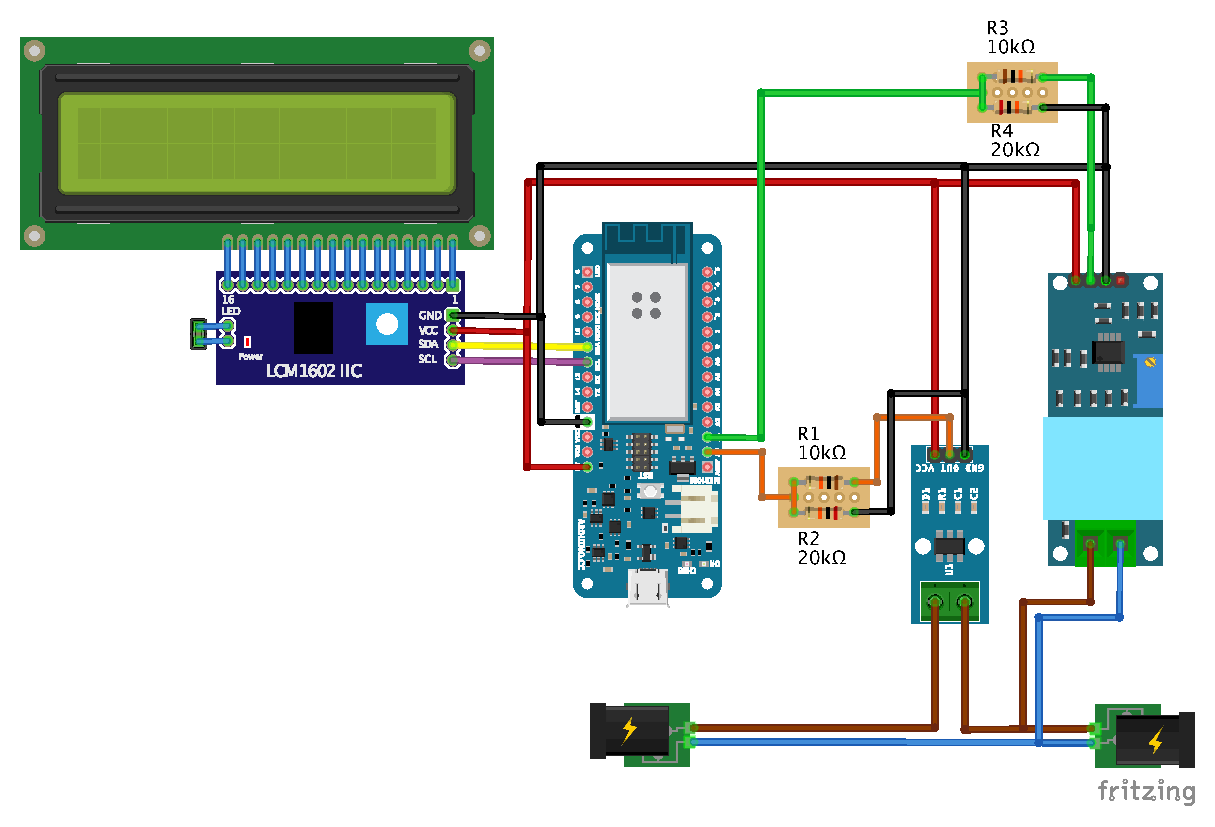
\includegraphics[width=\textwidth]{power_meter_bb.pdf}
\centering
\end{figure}

\subsection{Arduino MKR 1000 WiFi}
La scheda Arduino MKR 1000 WiFi è un prodotto specifico per IoT.
Integra al suo interno un processore Arm Cortex-M0 32-bit SAMD21, un chip di sicurezza ATECC508A e un controller Wi-Fi ATWINC1500.
Ci sono 7 pin d'ingresso analogico (A0-A6) in grado di rilevare una tensione d'ingresso compresa da 0 e 3.3V .

\subsection{Sensore di corrente}
Il sensore di corrente è un modulo che utilizza il sensore ACS712 in grado di misurare correnti fino a 5A.
Quando nessuna corrente attraversa il sensore ACS712, il modulo ha una tensione d'uscita pari a metà della tensione di alimentazione, che deve essere 5V.

Nel modello usato in questo progetto, la tensione di uscita varia di 185 mV per ogni A di corrente rilevata dal sensore.

\subsection{Sensore di tensione}
Il sensore di tensione è un modulo che utilizza il trasformatore ZMPT101B ed è in grado di misurare tensioni fino a 250V AC.
Sulla scheda è presente un potenziometro multigiro per regolare il guadagno dell'uscita ADC.

Quando non è presente nessuna tensione all'ingresso del trasformatore, il modulo ha una tensione d'uscita pari a metà della tensione di alimentazione che, anche in questo caso, deve essere 5V.

\subsection{Display LCD}
Per visualizzare i valori di tensione e corrente misurati dai sensori e quelli di potenza (reale ed apparente) calcolati, è stato utilizzato un display LCD da 16 caratteri e 2 righe.
Il display è pilotato da un modulo LM1602, basato sul chip PCF8574, che permette la connessione di qualunque scheda Arduino attraverso il bus $I^2C$.
Anche questo modulo deve essere alimentato a 5V.

\newpage

\subsection{Divisori di tensione}
I pin d'ingresso analogico della scheda Arduino MKR 1000 WiFi sono in grado di rilevare tensioni fino a 3.3V, mentre i sensori di corrente e tensione funzionano con una tensione di alimentazione di 5V.
Entrambi i sensori hanno una tensione di uscita che varia da 0 a 5V, incompatile con i pin della scheda Arduino.
Per ovviare al problema sono stati realizzati dei divisori di tensione (figura~\ref{fig:voltage_divider}) in modo da \textit{convertire} il range della tensione di uscita dei sensori da 0-5V a 0-3.3V.

\begin{figure}[h]
	\centering
	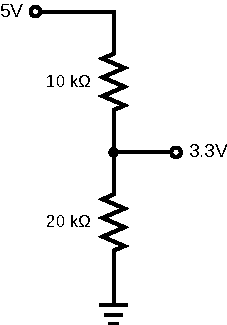
\includegraphics[width=0.25\textwidth]{voltage_divider.pdf}
	\caption{Divisore di tensione}
	\label{fig:voltage_divider}
\end{figure}

\newpage

\section{Codice Arduino}
Nella fase di \textit{setup}, vengono letti i valori di calibrazione dei sensori (argomento trattato in questa sezione), connessa la scheda alla rete Wi-Fi e attivato il display LCD.

Prima di attivare la connessione con il broker MQTT, viene generato il \textit{clientID} a partire da un prefisso (\emph{pwrmtr}) e dal valore del terzo e quarto ottetto dell'indirizzo IP.
Se necessario, vengono aggiunti degli zeri ai valori degli ottetti, in modo da ottenere un \textit{clientID} di lunghezza fissa 
In questo modo è possibile collegare circa 65.000 unità senza modificare il codice sorgente.
Per evitare connessioni al broker da parte di client non autorizzati, la connessione è autenticata tramite \textit{username} e \textit{password}.

Nella fase di \textit{loop}, sul display viene visualizzato il valore di corrente e tensione calcolato su una media di 1000 campioni.
Dato che le grandezze misurate dai sensori sono corrente e tensione alternata, per ottenere una misura accurata è stato necessario calcolarne il \emph{valore efficace} (semplificando, il valore equivalente in corrente continua).
Ogni milli secondo viene registrato un campione e ogni mille campioni (ogni secondo) viene calcolato il valore RMS dei campioni in questo modo:
\begin{itemize}
  \item si eleva al quadrato ogni campione, in modo da perdere il segno dei valori negativi
  \item si calcola la media dei quadrati dei campioni
  \item si estrae la radice quadrata della media
\end{itemize}

\noindent Per effettuare queste operazioni è stata usata la libreria Statistical\footfullcite{statistical}.

Sul display sono visualizzati anche i valori di potenza, calcolati su una media di 1000 campioni.
Per ottenere il valore di potenza reale viene fatta la media dei prodotti del valore istantaneo di corrente e tensione dei campioni.
L'unità di misura di questo valore è il Watt.
Mentre per ottenere il valore di potenza apparente viene fatta la media dei prodotti del valore efficace (RMS) di corrente e tensione calcolati in precedenza.
In questo caso l'unità di misura è il Volt Ampere(VA).

\newpage

Una volta ottenuti tutti i valori, questi vengono inviati al broker MQTT usando un \emph{topic} diverso per ogni valore:

\begin{enumerate}
  \item[]sensors/\textit{clientId}/voltage
  \item[] sensors/\textit{clientId}/current
  \item[] power/\textit{clientId}/real
  \item[] power/\textit{clientId}/apparent
\end{enumerate}

\subsection{Calibrazione}

The sensor module is a sensitive sensor. The output reading of the sensor might produce electrical noises or fake values even when there is no voltage detected. In order to greatly reduce this phenomenon, multiple samples must be taken for averaging and initial offset must be done.  
The second problem could be the false signal and accuracy problem. Each sensor has its own deviation error. When there is no voltage sensed, the sensor might not be 100% at middle point of voltage value. Some might be remaining at few milli voltages above / below the middle point even though after averaging. This might be due to voltage supplied not in exact 5V or due to the sensor itself. Thus 12V power adapter to power the Arduino UNO is highly recommended.

Besides, the sensor requires initial offset setting. You may need to manually offset the value by checking the false value when no voltage measurement during Arduino startup and then key in offset value in the code file. Secondly, make sure the sensor cables are tight because minor movement of wires might affects on the wire terminal connections thus affecting the accuracy reading.

Once the wave swing is calibrated to oscillate at exact middle point, after the calculation of squared, averaging and square root, there is still some minor false value existed even no voltage measurement. So our code included the second offset setting to eliminate this noise value. 


If you really read through the codes, we actually has reduced the potential wave amplitude by a factor of 0.66. 

RMSVoltageMean = (sqrt(voltageMean))*1.5;

What I realized is that by default, the waveform will start to distort before reaching 250Vac. It will affect the accuracy of other values if we calibrate based on distorted wave. So to solve this issue, I have reduced the amplitude by a factor of 0.66 in the coding, so that the waveform will not stretched till the maximum extend. You will realize when monitoring voltage is switched on, the voltage value is high and you need to reduce it. 




you can use the flash of the SAMD with the EEPROM emulation library

Microchip ATECC508A

10 Kb EEPROM Memory for Keys, Certificates, and Data


blocco di 32 bytes perchè The Read/Write command reads words (one four byte word or an 8-word block of 32 bytes)

The Write command writes either one four byte word or an 8-word block of 32 bytes to one of the
EEPROM zones on the device.

I would use a union because then the data exists in two different formats at the same time without any need for conversion.

slot 8 Typical Use Data Bytes 416





The output signal of the Single Phase AC Voltage Module is a waveform of analog values from 0 to 1023. The frequency of the wave is following the Voltage measured. Since the amplitude is adjustable, the voltage analog signal need to be calibrated. In order to calibrate, you need another voltmeter for reference. It can be either multimeter or regular voltmeter that can measure AC Voltage (RMS). The maximum voltage that the module can measured (250Vac) is referring to the Root Mean Square (RMS) value. Technically it can measure the waveform up to the peak at 353.55 Vac peak. 

The AC Voltage Module analog measurement is similar to Current Module. The voltage value will fluctuate up and down within 0 to 5V (0 to 1023 value). When no voltage detected, it will send analog signal at half the supply voltage (example 2.5V) which is about value 512. Different module will have different deviation error. Some might be reading exactly 512 when no measurement voltage detected but some may be slightly more or slightly less than value 512. You will have to manually key in the offset value during the first start or during no voltage detected. The AC Voltage Module requires at least 5V power supply and the signal output voltage is within 5V thus if you have a Arduino Nano or NodeMCU that have 3.3V analog pins, you need to add a voltage divider resistors in between to reduce or step down the output analog values.


\end{document}
